\documentclass{article}
\usepackage{physics}
\usepackage{amsmath}
\usepackage{graphicx}

\graphicspath{{./figs/}}

\title{Computatonal physics - Statistical Physics}
\author{Martin Johnsrud}

\begin{document}
    \maketitle
    
    \section*{Introduction}
    By numerically integrating Newtons equation of motion og many particles, confined to a box and interacting via the Leonard-Jones potential, it is possible to see the emergence of statistical behvior like the Maxwell-Boltzmann distribution. In this exercice, we explor this behavior, and ... (more to come)

    \section*{Single particel}
        A single particel with position $\vec x = (x_1, x_2)$ in a box is modeled in a potential 
        \begin{equation*}
            V_w(\vec x) = 
            \begin{cases}
                \frac{1}{2}K(r - R)^2, & r > R \\
                0, & r < R,
            \end{cases}
        \end{equation*}
        where $r = |\vec x|$. This leads to a force 
        \begin{equation*}
            \vec F_w(\vec x) = -\nabla V_w(\vec x) = 
            \begin{cases}
                -K(r - R)\hat x, & r>R \\
                0, & r<R.
            \end{cases}
        \end{equation*}
        This equiations can the numerically integrated to simulate the trajectory of the particle. This project is done using verlet integration, 
        \begin{align*} 
            & \vec x(t + \Delta t) = \vec x(t) + \dot{\vec x}(t) \Delta t + \frac{1}{2} F\big(\vec x(t)\big) \Delta t \\
            & \dot{\vec x}(t + \Delta t) = \dot{\vec x}(t) + \frac{1}{2} \Big[\Sigma \vec F\big(\vec x(t)\big) + \Sigma \vec F\big(\vec x(t + \Delta t)\big)\Big] \Delta t^2
        \end{align*}
        
        \begin{figure}
            
            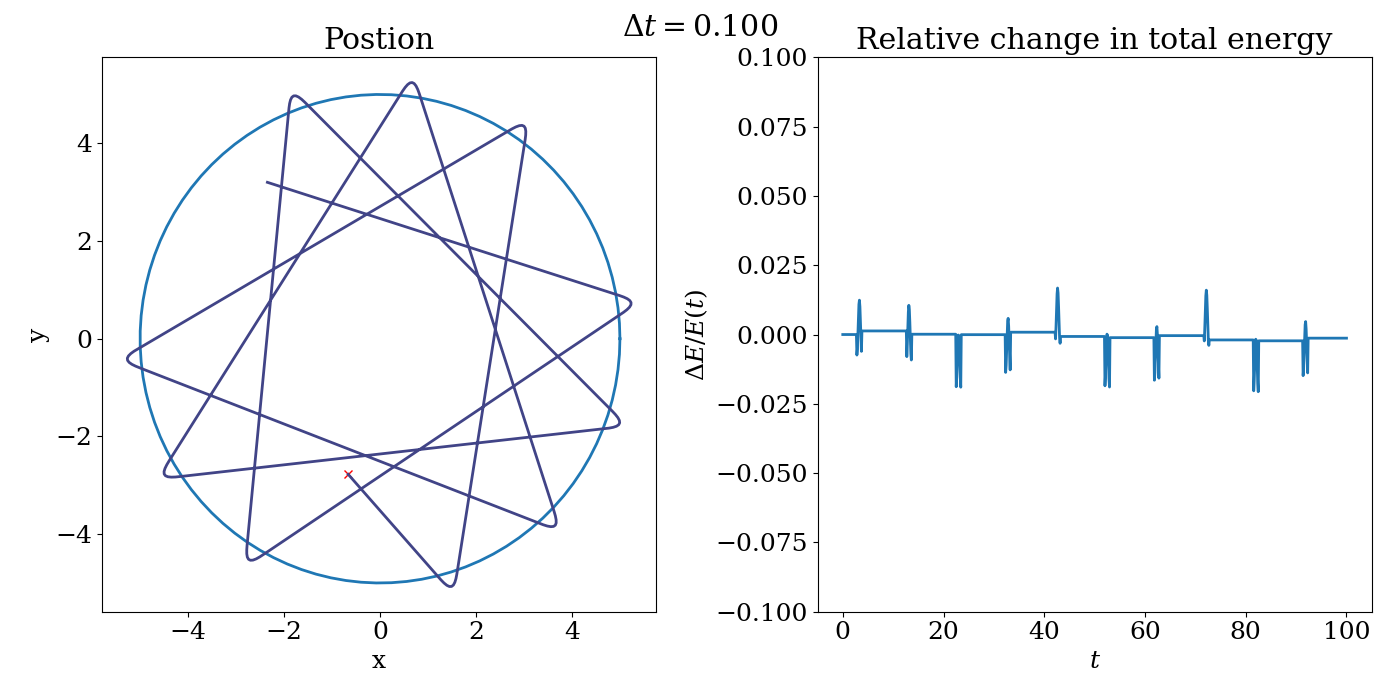
\includegraphics[width = \textwidth]{one_particle_01}
            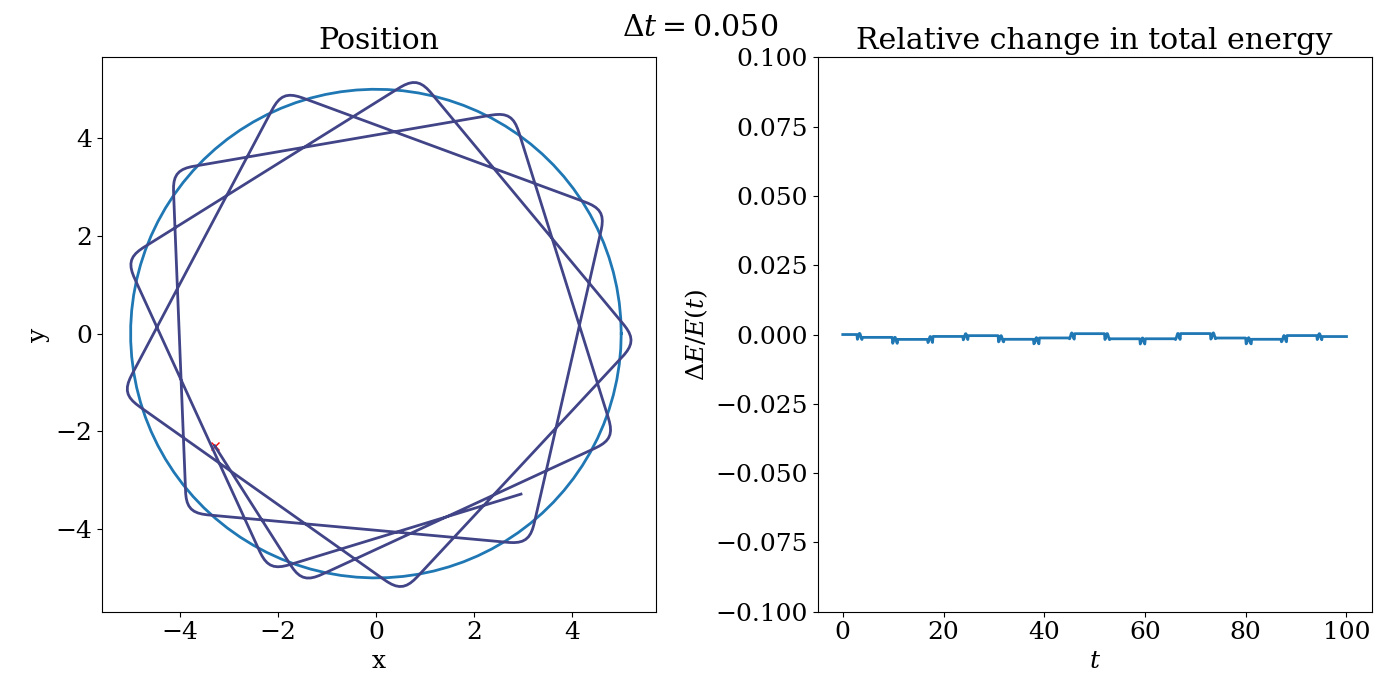
\includegraphics[width = \textwidth]{one_particle_005}
            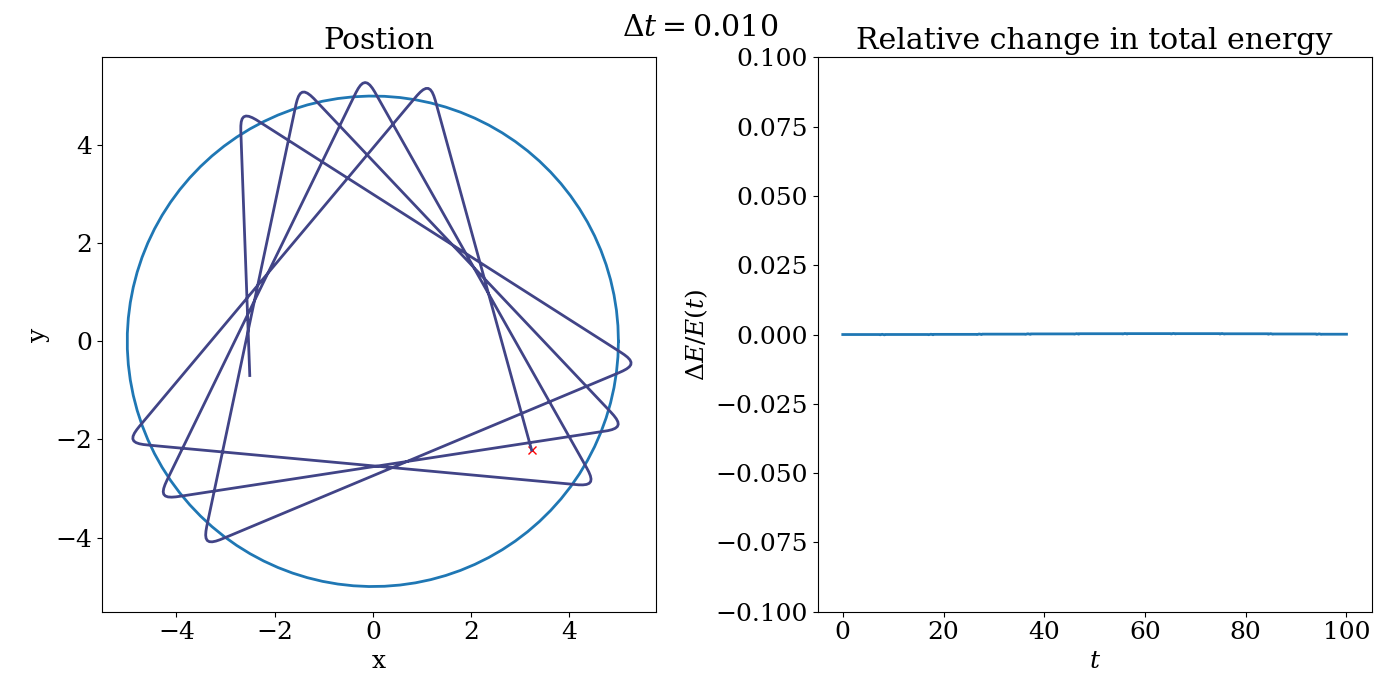
\includegraphics[width = \textwidth]{one_particle_001}

        \end{figure}

        Everything is done in units defined by the parametres $K, R$ and $\epsilon$, so that mass of the particle dissapears from the equations.

        \paragraph*{}
        

    \section*{$N$ particles}
        When moddeling $N$ particles $\{ \vec x_k\} = \{ (x_1^{(k)}, x_2^{(k)}) \}$, each one of them is subject to the force from the potential $V_w(\vec x_k)$, as well as a modified Leonard-Jones potential the interaction potential. The potential felt by particle $k$ is then
        \begin{equation*}
            V_k(\vec x_j) = 
            \sum_{r_{kj}<a}\epsilon \bigg[ \bigg( \frac{a}{r_{kj}}\bigg)^{12} - 2\bigg(\frac{a}{r_{kj}}\bigg)^{6} + 1 \bigg]
        \end{equation*}
        Here, $r_{kj} = |\vec x_k - \vec x_j|$. The force on particel $k$ by this potential is
        \begin{equation*}
            F_k (\vec x_j) = -\nabla_k V(\vec x_j) = \sum_{r_{kj}<a} 12 \epsilon \bigg[ \bigg( \frac{a}{r_{kj}}\bigg)^{12} - \bigg(\frac{a}{r_{kj}}\bigg)^{6}\bigg] \frac{\hat x_{kj}}{r_{kj}},
        \end{equation*}
        where $\hat x_{kj} = (\vec x_k - \vec x_j) / r_{kj}$
\end{document}